% Made up for the tikra benchmark.
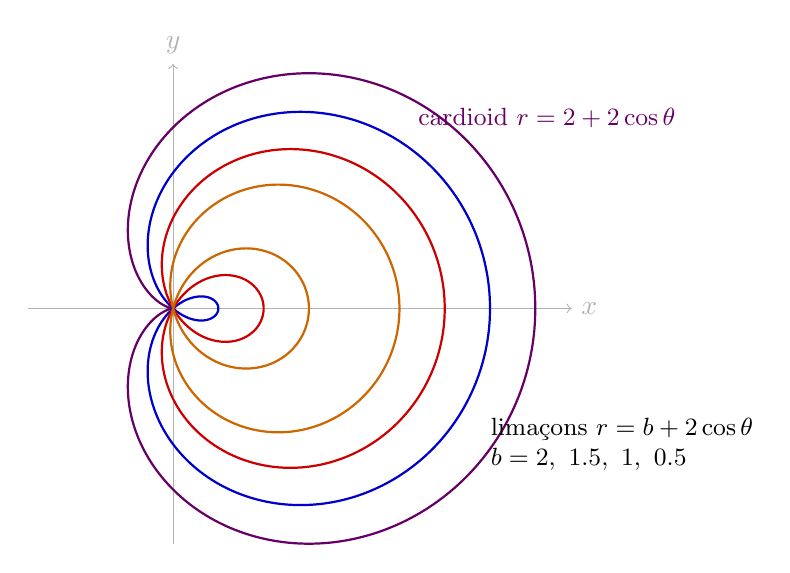
\begin{tikzpicture}[scale=1.15]
  \draw[gray!60, ->] (-1.6,0) -- (4.4,0) node[right] {$x$};
  \draw[gray!60, ->] (0,-2.6) -- (0,2.7) node[above] {$y$};
  \foreach \b/\c in {2/violet, 1.5/blue, 1/red, 0.5/orange} {
    \draw[\c!80!black, thick, smooth, domain=0:360, samples=180, variable=\t]
      plot ({(\b + 2*cos(\t))*cos(\t)}, {(\b + 2*cos(\t))*sin(\t)});
  }
  \node[violet!80!black, font=\small, anchor=west] at (2.6,2.1) {cardioid $r = 2 + 2\cos\theta$};
  \node[font=\small, align=left, anchor=west] at (3.4,-1.5)
    {lima\c{c}ons $r = b + 2\cos\theta$\\$b = 2,\ 1.5,\ 1,\ 0.5$};
\end{tikzpicture}
